\chapter{التعبير المورّثي: الاستنساخ والترجمة}\label{ch:b1:gene-expression}

تُقرأ \omterm{def:b1:genomes:gene}{مورّثة} من ثلاثين ألف \omterm{thm:b1:nucleic-acids:helix}{زوج قواعد} في ربع ساعة إلى نسخة عاملة،
وتُختصر إلى ألفي حرف، وتُشحن خارج \omterm{def:b1:eukaryotic-cell:nucleus}{النواة}، ويترجمها خمسة وعشرون
ريبوزومًا معًا إلى \omterm{def:b1:proteins:peptide}{بروتين} من خمسمئة \omterm{def:b1:proteins:aminoacid}{حمض أميني} --- واحدًا كل أربع
ثوانٍ، ما بقيت النسخة. وتنفق \omterm{def:b1:cell-unit-of-life:cell}{الخلية} على هذا طاقة أكثر مما تنفق على
أي شيء آخر تفعله. ويتتبع هذا الفصل المعلومة من \omterm{def:b1:nucleic-acids:chain}{DNA} إلى \omterm{def:b1:proteins:peptide}{البروتين}:
استنساخ \omterm{def:b1:genomes:gene}{المورّثة} إلى \omterm{def:b1:nucleic-acids:chain}{RNA}، وتحرير هذه النسخة في \omterm{def:b1:cell-unit-of-life:prokeuk}{حقيقيات النواة}،
والشفرة التي تربط ثلاثيات القواعد \omterm{def:b1:proteins:aminoacid}{بالأحماض الأمينية}، \omterm{def:b1:gene-expression:ribosome}{والريبوزوم}
الذي يقرؤها، وما يحدث \omterm{def:b1:proteins:peptide}{للبروتين} بعد صنعه.

\section{من المورّثة إلى البروتين}

\begin{proposition}[مسار المعلومة]\label{prop:b1:gene-expression:dogma}
\index{تعبير مورّثي}\index{استنساخ}\index{ترجمة}
تسير المعلومة الوراثية من \omterm{def:b1:nucleic-acids:chain}{DNA} إلى \omterm{def:b1:nucleic-acids:chain}{RNA} إلى \omterm{def:b1:proteins:peptide}{البروتين}. و\emph{الاستنساخ}
ينسخ إحدى خصلتي \omterm{def:b1:genomes:gene}{المورّثة} إلى \omterm{def:b1:nucleic-acids:chain}{RNA} تسلسله تسلسل الخصلة الأخرى (مع U
مكان T)؛ و\emph{الترجمة} تقرأ \omterm{def:b1:nucleic-acids:rnas}{RNA الرسول} ثلاث قواعد في كل مرة
وتركّب \omterm{def:b1:proteins:aminoacid}{الأحماض الأمينية} الموافقة في \omterm{def:b1:proteins:peptide}{عديد ببتيد}. وكل خطوة تستعمل
ازدواج القواعد: \omterm{def:b1:nucleic-acids:chain}{DNA} مع \omterm{def:b1:nucleic-acids:chain}{RNA} في الاستنساخ، والرسول مع RNA الناقل في
الترجمة. فتسلسل \omterm{def:b1:proteins:peptide}{البروتين} إذن نسخة من تسلسل مورّثته، وتغيّر \omterm{def:b1:nucleic-acids:nucleotide}{قاعدة}
واحدة قد يغيّر حمضًا أمينيًا واحدًا --- وهي الصلة بين الطفرة والنمط
الظاهري. ولا تعود المعلومة من \omterm{def:b1:proteins:peptide}{البروتين} إلى \omterm{def:b1:nucleic-acids:chain}{الحمض النووي}؛ والخطوة
العكسية الوحيدة، وهي نسخ \omterm{def:b1:nucleic-acids:chain}{RNA} إلى \omterm{def:b1:nucleic-acids:chain}{DNA} في \omterm{def:b1:genomes:virus}{الفيروسات} القهقرية، لا تمس
\omterm{def:b1:proteins:peptide}{البروتين}.
\end{proposition}

\section{الاستنساخ}

\begin{definition}[بوليميراز RNA، والمروّج، والاستنساخ]\label{def:b1:gene-expression:transcription}
\index{بوليميراز RNA}\index{مروّج}
\emph{بوليميراز \omterm{def:b1:nucleic-acids:chain}{RNA}} يخلّق \omterm{def:b1:nucleic-acids:chain}{RNA} على قالب من \omterm{def:b1:nucleic-acids:chain}{DNA}، من $5' \to 3'$،
انطلاقًا من ثلاثيات فوسفات النوكليوزيدات الريبية الأربعة، دون
بادئة. ويبدأ عند \emph{مروّج}، وهو تسلسل يقع أعلى المجرى من
\omterm{def:b1:genomes:gene}{المورّثة} مباشرة يتعرفه ويرتبط به؛ وفي البكتيريا تتولى التعرف وحدة
فرعية تسمى $\sigma$ (\emph{سيغما})، عند شريطين محفوظين على بعد
عشرة أزواج وخمسة وثلاثين زوجًا قبل موضع البداية. ويفتح \omterm{def:b1:enzymes:enzyme}{الإنزيم} نحو
خمسة عشر زوجًا من اللولب في \emph{فقاعة استنساخ}، وينسخ
\emph{الخصلة القالب} (تُقرأ $3' \to 5'$) إلى \omterm{def:b1:nucleic-acids:chain}{RNA} مطابق في التسلسل
للخصلة الأخرى، \emph{المشفِّرة}، ويتحرك على طولها بنحو خمسين
نوكليوتيدًا في الثانية، معيدًا إغلاق اللولب خلفه؛ وينسلخ \omterm{def:b1:nucleic-acids:chain}{RNA} وهو
يُصنع. ويقف عند \emph{تسلسل إنهاء}: وهو في البكتيريا تسلسل متمم
لنفسه ينطوي \omterm{def:b1:nucleic-acids:chain}{RNA} الموافق له في دبوس شعر يسحب النسخة حرة. وتستطيع
بوليميرازات كثيرة أن يتبع بعضها بعضًا على \omterm{def:b1:genomes:gene}{مورّثة} واحدة، فتُبدأ نسخة
كل ثانية.
\end{definition}

\begin{omfigure}
\begin{tikzpicture}[font=\footnotesize, >=Stealth, line cap=round]
  % DNA duplex left and right of bubble
  \draw[very thick, omDef] (0,0.5) -- (3.0,0.5); \draw[very thick, omDef!50] (0,-0.5) -- (3.0,-0.5);
  \draw[very thick, omDef] (8.0,0.5) -- (11.5,0.5); \draw[very thick, omDef!50] (8.0,-0.5) -- (11.5,-0.5);
  \foreach \x in {0.4,0.9,...,2.9} { \draw[gray!60] (\x,0.5) -- (\x,-0.5); }
  \foreach \x in {8.4,8.9,...,11.4} { \draw[gray!60] (\x,0.5) -- (\x,-0.5); }
  % bubble: strands separate
  \draw[very thick, omDef] (3.0,0.5) .. controls (4.0,1.3) and (7.0,1.3) .. (8.0,0.5);
  \draw[very thick, omDef!50] (3.0,-0.5) .. controls (4.0,-1.3) and (7.0,-1.3) .. (8.0,-0.5);
  % polymerase
  \draw[thick, omProp!80!black, fill=omProp!25, opacity=0.85] (5.5,0) ellipse (2.3 and 1.7);
  \node[omProp!80!black, anchor=east] at (2.7,1.5) {بوليميراز RNA}; \draw[omProp!80!black] (2.75,1.45) -- (3.6,1.0);
  % RNA transcript: paired to template in bubble, then exiting
  \draw[very thick, omThm] (4.0,-0.85) .. controls (5.0,-0.75) .. (6.0,-0.75) .. controls (6.5,-0.4) and (6.3,1.2) .. (5.2,2.3);
  \node[omThm, anchor=south] at (5.1,2.35) {RNA، النهاية $5'$ تبرز};
  \draw[thin, omThm] (6.0,-0.8) -- (6.4,-1.95);
  \node[omThm, anchor=north, font=\scriptsize] at (6.4,-2.0) {$3'$: النهاية النامية من RNA};
  % labels
  \node[anchor=east, omDef] at (-0.1,0.5) {$5'$ الخصلة المشفِّرة $3'$};
  \node[anchor=east, omDef!70!black] at (-0.1,-0.5) {$3'$ الخصلة القالب $5'$};
  \draw[->, very thick, omProp!80!black] (8.6,1.9) -- (10.2,1.9) node[midway, above] {اتجاه الاستنساخ};
  \node[anchor=north, align=center, gray] at (5.5,-2.55) {RNA متمم للخصلة القالب ومطابق (مع U مكان T) للخصلة المشفِّرة؛\\ نحو خمسة عشر زوج قواعد مفتوحة في كل لحظة، ويعود اللولب إلى الانغلاق خلف الإنزيم};
\end{tikzpicture}

{\small الاستنساخ. يفتح البوليميراز فقاعة، ويزاوج \omterm{def:b1:nucleic-acids:nucleotide}{النوكليوتيدات}
الريبية مع الخصلة القالب ويصلها من $5' \to 3'$؛ ويغادر \omterm{def:b1:nucleic-acids:chain}{RNA} عبر \omterm{def:b1:membranes-transport:transporters}{قناة}
\omterm{def:b1:enzymes:enzyme}{والإنزيم} يتقدم.}
\end{omfigure}

\begin{proposition}[الاستنساخ ومعالجة RNA في حقيقيات النواة]\label{prop:b1:gene-expression:processing}
\index{تشذيب}\index{RNA الرسول}\index{قلنسوة}\index{ذيل عديد الأدنين}
\omterm{def:b1:cell-unit-of-life:prokeuk}{لحقيقيات النواة} ثلاثة بوليميرازات: I لأنواع \omterm{def:b1:nucleic-acids:rnas}{RNA الريبوزومي} الكبيرة،
وII لأنواع \omterm{def:b1:nucleic-acids:rnas}{RNA الرسول}، وIII لأنواع RNA الناقل \omterm{def:b1:nucleic-acids:chain}{وRNA} الصغيرة.
والبوليميراز II لا يتعرف مروّجه وحده: بل تتجمع عليه مجموعة من
\emph{عوامل الاستنساخ العامة} (عند تسلسل TATA على بعد نحو ثلاثين
زوجًا أعلى المجرى في \omterm{def:b1:genomes:gene}{مورّثات} كثيرة) فتستقدم \omterm{def:b1:enzymes:enzyme}{الإنزيم}، وتعدّل \omterm{def:b1:proteins:peptide}{بروتينات}
منظِّمة مرتبطة قريبًا أو بعيدًا سرعةَ العملية
(\cref{ch:b1:expression-control}). وتُعالَج النسخة الأولية
(\emph{معالجةً}) في \omterm{def:b1:eukaryotic-cell:nucleus}{النواة}: تُضاف \emph{قلنسوة} من غوانين معدَّل إلى
النهاية $5'$، وذيل من نحو مئتي أدنين (\emph{عديد الأدنين}) إلى
النهاية $3'$، وتُزال \omterm{def:b1:genomes:gene}{الإنترونات} في عملية \emph{التشذيب} --- إذ
يتعرف معقد من أنواع \omterm{def:b1:nucleic-acids:chain}{RNA} صغيرة \omterm{def:b1:proteins:peptide}{وبروتينات}، هو \emph{الجسيم
المشذِّب}، GU عند بداية كل \omterm{def:b1:genomes:gene}{إنترون} وAG عند نهايته، فيقص ويصل
\omterm{def:b1:genomes:gene}{الإكسونات}. وعندئذ فقط يُصدَّر الرسول الناضج إلى \omterm{def:b1:eukaryotic-cell:organelle}{العصارة الخلوية}. وكثير من
\omterm{def:b1:genomes:gene}{المورّثات} يُشذَّب بأكثر من طريقة (\emph{تشذيب بديل})، فتعطي \omterm{def:b1:genomes:gene}{المورّثة}
الواحدة عدة \omterm{def:b1:proteins:peptide}{بروتينات}؛ \omterm{def:b1:genomes:gene}{فمورّثات} الإنسان العشرون ألفًا تصنع نحو مئة
ألف.
\end{proposition}
\begin{proof}[شواهد]
هجّن شارب وروبرتس (1977) \omterm{def:b1:nucleic-acids:chain}{RNA} رسولًا فيروسيًا مع \omterm{def:b1:nucleic-acids:chain}{DNA} مورّثته ونظرا
إلى الهجائن \omterm{prop:b1:cell-unit-of-life:microscopes}{بالمجهر الإلكتروني}: ازدوج \omterm{def:b1:nucleic-acids:chain}{RNA} مع \omterm{def:b1:nucleic-acids:chain}{DNA} في عدة شرائط،
وبينها انعقد \omterm{def:b1:nucleic-acids:chain}{DNA} في عرى غير مزدوجة --- وهي \omterm{def:b1:genomes:gene}{الإنترونات}، الحاضرة في
\omterm{def:b1:genomes:gene}{المورّثة} الغائبة عن الرسول. أما \omterm{def:b1:genomes:gene}{المورّثات} البكتيرية، وقد عوملت
المعاملة نفسها، فلم تعطِ عرى. وحجم النسخة الأولية \omterm{def:b1:genomes:gene}{للمورّثة}، مقيسًا
في \omterm{def:b1:eukaryotic-cell:nucleus}{النواة}، يوافق \omterm{def:b1:genomes:gene}{المورّثة}؛ وحجم الرسول السيتوبلازمي يوافق
\omterm{def:b1:genomes:gene}{الإكسونات} وحدها.
\end{proof}

\begin{omfigure}
\begin{tikzpicture}[font=\footnotesize, >=Stealth, line cap=round]
  % gene
  \draw[very thick, gray] (0,3.2) -- (11,3.2);
  \fill[omDef!70] (0.6,2.95) rectangle (1.8,3.45); \fill[omDef!70] (4.2,2.95) rectangle (5.4,3.45); \fill[omDef!70] (8.0,2.95) rectangle (9.6,3.45);
\node[anchor=east] at (-0.1,3.2) {مورّثة};
\node[anchor=south, font=\scriptsize] at (1.2,3.5) {إكسون 1}; \node[anchor=south, font=\scriptsize] at (4.8,3.5) {إكسون 2}; \node[anchor=south, font=\scriptsize] at (8.8,3.5) {إكسون 3};
  \draw[->, thick] (5.5,2.7) -- (5.5,2.2) node[midway, right] {استنساخ};
  % primary transcript
  \draw[very thick, omThm!60] (0.6,1.8) -- (9.6,1.8);
  \fill[omDef!70] (0.6,1.6) rectangle (1.8,2.0); \fill[omDef!70] (4.2,1.6) rectangle (5.4,2.0); \fill[omDef!70] (8.0,1.6) rectangle (9.6,2.0);
\node[anchor=east] at (-0.1,1.8) {النسخة الأولية};
\node[anchor=north, font=\scriptsize] at (3.0,1.55) {إنترون 1}; \node[anchor=north, font=\scriptsize] at (6.7,1.55) {إنترون 2};
  \draw[->, thick] (5.5,1.2) -- (5.5,0.7) node[pos=0.9, right, align=left] {قلنسوة، وتشذيب،\\ وإضافة عديد الأدنين};
  % mature mRNA
\fill[omExo!70] (0.2,0.15) circle (0.13); \node[anchor=south, font=\scriptsize] at (0.2,0.3) {قلنسوة};
  \fill[omDef!70] (0.4,0.0) rectangle (1.6,0.4); \fill[omDef!70] (1.6,0.0) rectangle (2.8,0.4); \fill[omDef!70] (2.8,0.0) rectangle (4.4,0.4);
\draw[very thick, omExo!70] (4.4,0.2) -- (6.0,0.2); \node[anchor=west, font=\scriptsize] at (6.05,0.2) {ذيل عديد الأدنين (AAAA\ldots)};
\node[anchor=east] at (-0.1,0.2) {الرسول الناضج};
\node[anchor=north, align=center, gray] at (5.5,-0.4) {الإكسونات موصولة بالترتيب؛ والإنترونات، وهي معظم النسخة، تُهضم في النواة};
\end{tikzpicture}

{\small من \omterm{def:b1:genomes:gene}{المورّثة} إلى الرسول في \omterm{def:b1:cell-unit-of-life:prokeuk}{حقيقية النواة}: تُستنسخ \omterm{def:b1:genomes:gene}{المورّثة}
كلها، ثم تُقص \omterm{def:b1:genomes:gene}{الإنترونات} وتوصل \omterm{def:b1:genomes:gene}{الإكسونات}، وتُضاف قلنسوة وذيل من
عديد الأدنين، ويغادر الرسول الناضج \omterm{def:b1:eukaryotic-cell:nucleus}{النواة}.}
\end{omfigure}

\section{الشفرة الوراثية}

\begin{definition}[الشفرة الوراثية]\label{def:b1:gene-expression:code}
\index{شفرة وراثية}\index{كودون}\index{إطار قراءة}
\emph{الشفرة الوراثية} تربط ثلاثيات من قواعد الرسول، وهي
\emph{الكودونات}، \omterm{def:b1:proteins:aminoacid}{بالأحماض الأمينية}. فمن الكودونات الأربعة والستين
يحدد واحد وستون \omterm{def:b1:proteins:aminoacid}{الأحماض الأمينية} العشرين، وثلاثة (UAA وUAG وUGA)
إشارات \emph{توقف}؛ وAUG يحدد الميثيونين وهو أيضًا كودون
\emph{البدء}، فكل \omterm{def:b1:proteins:peptide}{عديد ببتيد} جديد يبدأ بالميثيونين. والشفرة
\emph{منحلّة} --- فلأكثر \omterm{def:b1:proteins:aminoacid}{الأحماض الأمينية} عدة كودونات تختلف غالبًا
في الموضع الثالث --- و\emph{غير متراكبة}، تُقرأ بلا علامات ترقيم في
\emph{إطار قراءة} يثبته كودون البدء، و\emph{عامة} تقريبًا، هي نفسها
في البكتيريا والنباتات والحيوانات مع اختلافات طفيفة في \omterm{def:b1:eukaryotic-cell:mitochondrion}{المتقدرات}:
\omterm{def:b1:genomes:gene}{فمورّثة} بشرية تُوضع في بكتيريا تُقرأ قراءة صحيحة.
\end{definition}

\begin{omfigure}
\begin{center}
\footnotesize
\begin{tabular}{c|cccc|c}
\hline
\omterm{def:b1:nucleic-acids:nucleotide}{القاعدة} & \multicolumn{4}{c|}{\omterm{def:b1:nucleic-acids:nucleotide}{القاعدة} الثانية} & \omterm{def:b1:nucleic-acids:nucleotide}{القاعدة} \\
الأولى & U & C & A & G & الثالثة \\
\hline
U & Phe Phe Leu Leu & Ser Ser Ser Ser & Tyr Tyr \textbf{توقف} \textbf{توقف} & Cys Cys \textbf{توقف} Trp & U C A G \\
C & Leu Leu Leu Leu & Pro Pro Pro Pro & His His Gln Gln & Arg Arg Arg Arg & U C A G \\
A & Ile Ile Ile \textbf{Met} & Thr Thr Thr Thr & Asn Asn Lys Lys & Ser Ser Arg Arg & U C A G \\
G & Val Val Val Val & Ala Ala Ala Ala & Asp Asp Glu Glu & Gly Gly Gly Gly & U C A G \\
\hline
\end{tabular}
\end{center}

{\small \omterm{def:b1:gene-expression:code}{الشفرة الوراثية}. تسرد كل خانة \omterm{def:b1:gene-expression:code}{الكودونات} الأربعة ذات \omterm{def:b1:nucleic-acids:nucleotide}{القاعدة}
الأولى والثانية المعطاتين \omterm{def:b1:nucleic-acids:nucleotide}{والقاعدة} الثالثة U وC وA وG بهذا الترتيب.
وAUG هو الميثيونين وإشارة البدء؛ وUAA وUAG وUGA إشارات توقف. \omterm{def:b1:nucleic-acids:nucleotide}{والقاعدة}
الثالثة كثيرًا ما لا تهم: فالشفرة منحلّة.}
\end{omfigure}

\begin{proposition}[كيف قُرئت الشفرة]\label{prop:b1:gene-expression:nirenberg}
الشفرة شفرة ثلاثية غير متراكبة، ويمكن تعيين معنى كل \omterm{def:b1:gene-expression:code}{كودون} فيها
بالكيمياء.
\end{proposition}
\begin{proof}[شواهد]
أحدث كريك وبرينر (1961) في \omterm{def:b1:genomes:gene}{مورّثة} عاثية طفرات تضيف \omterm{def:b1:nucleic-acids:nucleotide}{قاعدة} واحدة أو
تحذفها: فأتلف تغيير واحد منها وظيفة \omterm{def:b1:genomes:gene}{المورّثة}، وأتلفها تغييران، لكن
ثلاث إضافات (أو ثلاثة حذوف) متقاربة أعادتها --- فالرسول يُقرأ
ثلاثات، من نقطة بداية ثابتة، والإضافة تزيح إطار كل ما بعدها. وأضاف
نيرنبرغ وماتاي (1961) \omterm{def:b1:nucleic-acids:chain}{RNA} اصطناعيًا من اليوراسيل وحده إلى مستخلص
خالٍ من \omterm{def:b1:cell-unit-of-life:cell}{الخلايا} من \emph{E. coli} مع \omterm{def:b1:proteins:aminoacid}{الأحماض الأمينية} العشرين: فصنع
سلسلة من الفينيل ألانين وحده، فالثلاثي UUU إذن يعني Phe؛ وأسندت رسائل
اصطناعية أخرى، ثم ارتباط ثلاثيات نوكليوتيدية مفردة \omterm{def:b1:gene-expression:ribosome}{بالريبوزومات} مع
أنواع RNA الناقل الخاصة بها، \omterm{def:b1:gene-expression:code}{الكودونات} الأربعة والستين جميعها بحلول
1966.
\end{proof}

\begin{example}[قراءة رسول]\label{ex:b1:gene-expression:reading}
الرسول $5'$-\ldots{}GC\underline{AUG}GCUUUCGGAUAA\ldots{}-$3'$
يُقرأ من AUG: هي AUG GCU UUC GGA UAA --- ميثيونين-ألانين-فينيل
ألانين-غليسين-توقف: ببتيد من أربع بقايا. واحذف G الأولى بعد AUG
ينزح الإطار: AUG CUU UCG GAU AA\ldots{} --- ميثيونين-لوسين-سيرين-
أسبارتات\ldots، وهو \omterm{def:b1:proteins:peptide}{بروتين} مختلف بطول مختلف. وغيّر UUC إلى UUU فلا
يتغير شيء: كلاهما Phe، وهي طفرة \emph{صامتة}.
\end{example}

\section{الترجمة}

\begin{definition}[RNA الناقل وإنزيمات شحنه]\label{def:b1:gene-expression:trna}
\index{RNA الناقل}\index{كودون مضاد}\index{إنزيم شحن RNA الناقل}
\emph{RNA الناقل} (\cref{ch:b1:nucleic-acids}) هو الوسيط بين \omterm{def:b1:gene-expression:code}{الكودون}
\omterm{def:b1:proteins:aminoacid}{والحمض الأميني}: فله \emph{\omterm{def:b1:gene-expression:code}{كودون} مضاد}، وهو ثلاث قواعد في عروة،
يزدوج مضاد التوازي مع \omterm{def:b1:gene-expression:code}{كودون} من الرسول، ونهايته $3'$ تحمل \omterm{def:b1:proteins:aminoacid}{الحمض
الأميني} الموافق. والازدواج في الموضع الثالث من \omterm{def:b1:gene-expression:code}{الكودون} رخو
(\emph{ترنّح})، فنحو أربعين نوعًا من RNA الناقل تكفي لواحد وستين
كودونًا. ويشحن كل RNA ناقل \emph{\omterm{def:b1:enzymes:enzyme}{إنزيم} شحن خاص به}، وهو \omterm{def:b1:enzymes:enzyme}{إنزيم} يتعرف
\omterm{def:b1:proteins:aminoacid}{الحمض الأميني} وRNA الناقل معًا ويصلهما في خطوتين بكلفة \omterm{def:b1:water-small-molecules:atp}{ATP} واحد
(يُشطر إلى AMP: أي رابطتان عاليتا الطاقة)، ويدقق في \omterm{def:b1:proteins:aminoacid}{الحمض الأميني}
وهو يفعل. وهذه \omterm{def:b1:enzymes:enzyme}{الإنزيمات} العشرون هي حيث تُنفَّذ الشفرة فعلًا: \omterm{def:b1:gene-expression:ribosome}{فالريبوزوم}
لا يتحقق من \omterm{def:b1:proteins:aminoacid}{الحمض الأميني} الذي يحمله RNA ناقل، بل من مطابقة كودونه
المضاد وحدها.
\end{definition}

\begin{definition}[الريبوزوم]\label{def:b1:gene-expression:ribosome}
\index{ريبوزوم}
\emph{الريبوزوم} جسيم من وحدتين فرعيتين، كل منهما من \omterm{def:b1:nucleic-acids:chain}{RNA} ريبوزومي
\omterm{def:b1:proteins:peptide}{وبروتينات} (في البكتيريا: وحدة صغيرة 30S ووحدة كبيرة 50S، معًا 70S،
\qty{2.5}{MDa}؛ وريبوزومات \omterm{def:b1:cell-unit-of-life:prokeuk}{حقيقيات النواة} أكبر، 80S). والوحدة
الصغيرة ترتبط بالرسول وتفك شفرته؛ والوحدة الكبيرة تمسك أنواع RNA
الناقل وتكوّن \omterm{def:b1:proteins:peptide}{الرابطة الببتيدية} --- والحفاز هو \omterm{def:b1:nucleic-acids:rnas}{RNA الريبوزومي} نفسه.
وثلاثة مواقع لأنواع RNA الناقل تمتد عبر الوحدتين: A (أمينوأسيل، حيث يدخل
RNA الناقل المشحون التالي)، وP (ببتيديل، يمسك السلسلة النامية)،
وE (الخروج).
\end{definition}

\begin{omfigure}
\begin{tikzpicture}
  \node[anchor=south west, inner sep=0] (img) at (0,0)
    {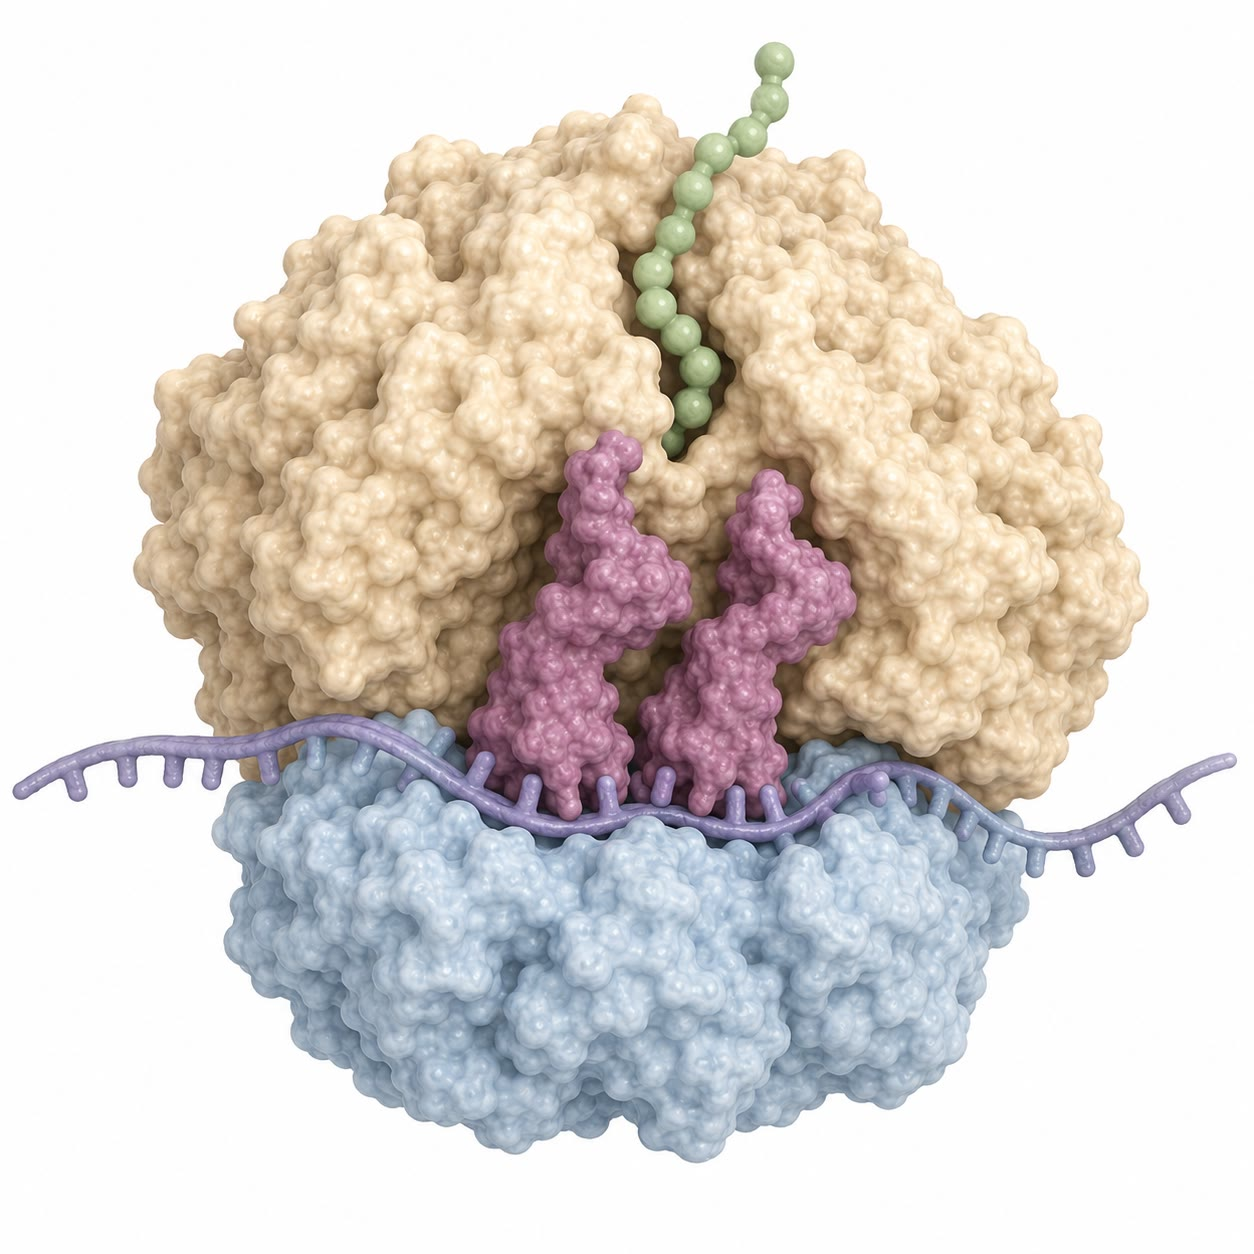
\includegraphics[width=0.46\linewidth]{images/book3/ai/fig-ribosome-3d.jpg}};
  \begin{scope}[x={(img.south east)}, y={(img.north west)},
      every node/.style={font=\small}]
    \draw[omDef, thick] (0.30,0.72) -- (0.30,1.08) node[above] {الوحدة الكبيرة: هنا تُصنع الرابطة الببتيدية};
    \draw[omDef, thick] (0.50,0.15) -- (0.50,-0.08) node[below] {الوحدة الصغيرة: تفك شفرة الرسول};
    \draw[omDef, thick] (0.47,0.52) -- (-0.03,0.44) node[left, align=right] {RNA ناقل في\\ الموقعين P وA};
    \draw[omDef, thick] (0.92,0.36) -- (1.03,0.26) node[right] {mRNA};
    \draw[omDef, thick] (0.57,0.88) -- (1.03,0.90) node[right, align=left] {عديد الببتيد يغادر\\ عبر نفق الخروج};
  \end{scope}
\end{tikzpicture}

{\small \omterm{def:b1:gene-expression:ribosome}{الريبوزوم}: وحدتان فرعيتان مطبقتان على الرسول، ونوعان من RNA
الناقل في الشق، والسلسلة النامية تغادر عبر نفق في الوحدة الكبيرة.}
\end{omfigure}

\begin{proposition}[دورة الاستطالة]\label{prop:b1:gene-expression:elongation}
تبدأ الترجمة حين تجد الوحدة الصغيرة \omterm{def:b1:gene-expression:code}{كودون} البدء --- في البكتيريا
بازدواج تسلسل من \omterm{def:b1:nucleic-acids:rnas}{RNA الريبوزومي} مع موقع أعلى المجرى من AUG مباشرة،
وفي \omterm{def:b1:cell-unit-of-life:prokeuk}{حقيقيات النواة} بالارتباط بالقلنسوة والمسح حتى أول AUG --- ويستقر
RNA الناقل البادئ (الميثيونين) في الموقع P؛ ثم تنضم الوحدة الكبيرة.
وتضيف كل دورة \emph{استطالة} بقية واحدة: فيسلّم عاملُ استطالة RNA
ناقلًا مشحونًا يوافق كودونُه المضاد كودونَ الموقع A ويُتحقق منه
(بكلفة GTP واحد)؛ وينقل \omterm{def:b1:nucleic-acids:rnas}{RNA الريبوزومي} في الوحدة الكبيرة السلسلة
النامية من RNA الناقل في الموقع P إلى \omterm{def:b1:proteins:aminoacid}{الحمض الأميني} في RNA الناقل في
الموقع A، فتتكون \omterm{def:b1:proteins:peptide}{الرابطة الببتيدية}؛ ويتحرك \omterm{def:b1:gene-expression:ribosome}{الريبوزوم} كودونًا واحدًا
(بكلفة GTP ثانٍ)، فينزاح نوعا RNA الناقل إلى P وE، ويغادر الفارغ.
وعند \omterm{def:b1:gene-expression:code}{كودون} توقف يدخل \emph{عامل تحرير} الموقع A فتُحلمأ السلسلة حرة.
وتضيف \omterm{def:b1:gene-expression:ribosome}{ريبوزومات} البكتيريا خمس عشرة إلى عشرين بقية في الثانية،
\omterm{def:b1:gene-expression:ribosome}{وريبوزومات} \omterm{def:b1:cell-unit-of-life:prokeuk}{حقيقيات النواة} اثنتين إلى خمس؛ وتقرأ عدة \omterm{def:b1:gene-expression:ribosome}{ريبوزومات} رسولًا
واحدًا معًا، مكوّنة \emph{عديد \omterm{def:b1:gene-expression:ribosome}{ريبوزوم}}.
\end{proposition}

\begin{omfigure}
\begin{tikzpicture}[font=\footnotesize, >=Stealth, line cap=round,
  rib/.style={draw, thick, rounded corners=8pt, fill=omDef!12, minimum width=30mm, minimum height=14mm},
  trna/.style={draw, thick, fill=omProp!30, minimum width=6mm, minimum height=9mm, inner sep=1pt, font=\scriptsize}]
  \foreach \i/\title in {0/{1. دخول RNA ناقل مشحون إلى الموقع A}, 1/{2. الرابطة الببتيدية: انتقال السلسلة إلى RNA الناقل في الموقع A}, 2/{3. الانزياح: تقدم الريبوزوم كودونًا واحدًا}} {
    \begin{scope}[xshift=\i*4.5cm]
      \node[rib] (r) at (0,0) {};
      \draw[very thick, omThm] (-2.0,-0.9) -- (2.0,-0.9);
      \node[font=\scriptsize] at (-0.45,-0.55) {P}; \node[font=\scriptsize] at (0.45,-0.55) {A};
      \node[anchor=north, align=center, font=\scriptsize, text width=40mm] at (0,-1.75) {\title};
    \end{scope}
  }
  % state 1: P holds chain, A receives new tRNA
  \node[trna] at (-0.45,0.05) {}; \draw[very thick, omExo!70!black] (-0.45,0.5) -- (-0.45,1.4); \foreach \y in {0.6,0.85,1.1,1.35} { \fill[omExo!70!black] (-0.45,\y) circle (0.09); }
  \node[trna] at (0.45,0.05) {}; \fill[omExo!70!black] (0.45,0.6) circle (0.09);
  \draw[->, thick, omProp!80!black] (1.6,1.3) -- (0.75,0.7); \node[font=\scriptsize, anchor=west] at (1.4,1.45) {GTP};
  % state 2: chain transferred
  \node[trna] at (4.05,0.05) {}; \node[trna] at (4.95,0.05) {}; \draw[very thick, omExo!70!black] (4.95,0.5) -- (4.95,1.65); \foreach \y in {0.6,0.85,1.1,1.35,1.6} { \fill[omExo!70!black] (4.95,\y) circle (0.09); }
  % state 3: translocated: chain on P, empty tRNA leaving at E, A free
  \node[trna, fill=gray!20] at (7.6,0.05) {}; \node[trna] at (8.55,0.05) {}; \draw[very thick, omExo!70!black] (8.55,0.5) -- (8.55,1.65); \foreach \y in {0.6,0.85,1.1,1.35,1.6} { \fill[omExo!70!black] (8.55,\y) circle (0.09); }
  \draw[->, thick, gray] (7.6,-0.4) -- (7.0,-1.0); \node[font=\scriptsize, gray, anchor=east] at (7.05,-0.4) {E};
  \draw[->, thick, omProp!80!black] (10.7,0.3) -- (10.7,-0.3); \node[font=\scriptsize, anchor=west] at (10.8,0.3) {GTP};
  \draw[->, thick, omThm] (9.4,-1.3) -- (10.4,-1.3) node[right, font=\scriptsize, omThm] {الرسول ينزاح};
\end{tikzpicture}

{\small دورة استطالة واحدة. يُقبل RNA ناقل مشحون في الموقع A حين
يطابق كودونه المضاد؛ ويصل \omterm{def:b1:nucleic-acids:rnas}{RNA الريبوزومي} السلسلة إلى حمضه الأميني؛
ويتقدم \omterm{def:b1:gene-expression:ribosome}{الريبوزوم} كودونًا واحدًا، ويغادر RNA الناقل الفارغ. أي GTP
اثنان لكل بقية، زائد الرابطتين عاليتي الطاقة المنفقتين في شحن RNA
الناقل.}
\end{omfigure}

\begin{omfigure}
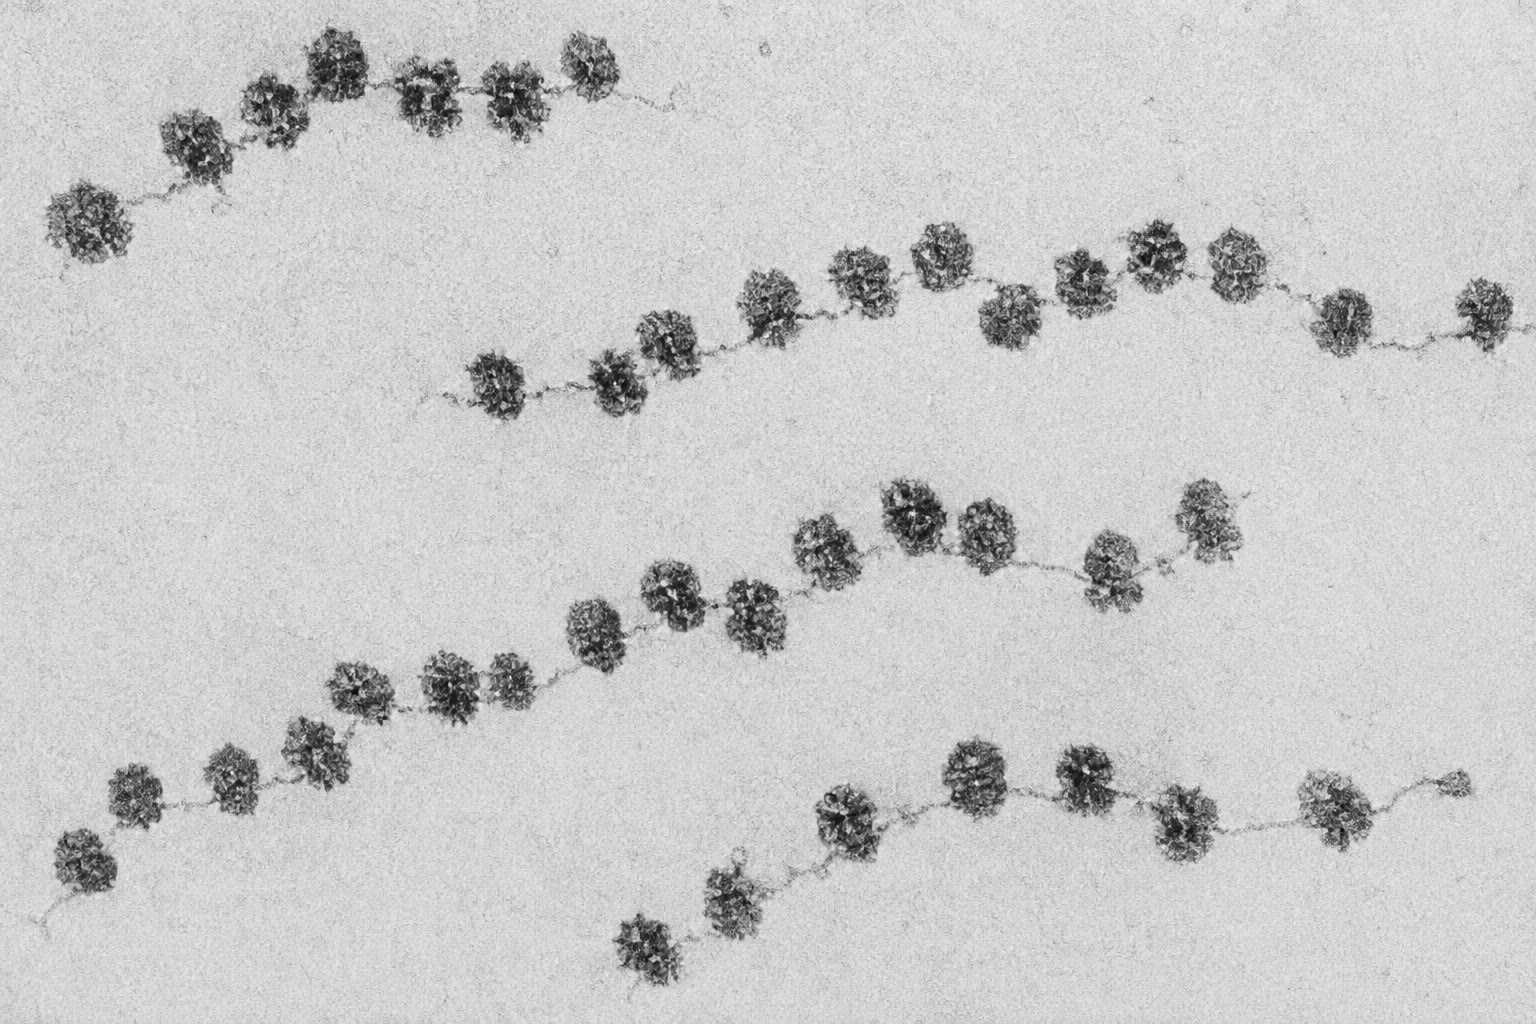
\includegraphics[width=0.5\linewidth]{images/book3/ai/b3-19-polysome-tem.jpg}

{\small عديدات \omterm{def:b1:gene-expression:ribosome}{الريبوزوم} تحت \omterm{prop:b1:cell-unit-of-life:microscopes}{المجهر الإلكتروني}: \omterm{def:b1:gene-expression:ribosome}{ريبوزومات} منظومة على
رسول، كل واحد منها يصنع نسخته من \omterm{def:b1:proteins:peptide}{البروتين}.}
\end{omfigure}

\begin{method}[حساب تخليق بروتين]\label{met:b1:gene-expression:reckon}
\begin{enumerate}
  \item الطول: \omterm{def:b1:proteins:peptide}{بروتين} من $n$ بقية يحتاج إلى تسلسل مشفِّر من
        $3n + 3$ \omterm{def:b1:nucleic-acids:nucleotide}{نوكليوتيد} (بما فيه \omterm{def:b1:gene-expression:code}{كودون} التوقف)، داخل رسول أطول
        منه بنهايتيه غير المترجمتين، وداخل \omterm{def:b1:genomes:gene}{المورّثة} أطول منه
        بإنتروناتها.
  \item الزمن: اقسم $n$ على سرعة الاستطالة (\qtyrange{15}{20}{}
        في الثانية في البكتيريا، و\qtyrange{2}{5}{} في \omterm{def:b1:cell-unit-of-life:prokeuk}{حقيقيات
        النواة})؛ ويقرأ الرسولَ \omterm{def:b1:gene-expression:ribosome}{ريبوزوم} كل \qtyrange{80}{100}{}
        \omterm{def:b1:nucleic-acids:nucleotide}{نوكليوتيد}، فالمردود لكل رسول سلسلة كل (المسافة / السرعة)
        ثانية.
  \item الطاقة: أربع روابط فوسفاتية عالية الطاقة لكل بقية (اثنتان
        لشحن RNA الناقل، وGTP اثنان على \omterm{def:b1:gene-expression:ribosome}{الريبوزوم})، زائد استنساخ
        الرسول باثنتين لكل \omterm{def:b1:nucleic-acids:nucleotide}{نوكليوتيد}، موزعًا على كل السلاسل التي
        يعطيها ذلك الرسول.
  \item الدقة: نحو \omterm{def:b1:proteins:aminoacid}{حمض أميني} خاطئ واحد في $10^4$ \omterm{def:b1:gene-expression:code}{كودون}؛ \omterm{def:b1:proteins:peptide}{فبروتين} من
        \qty{500}{} بقية يكون خاطئًا في موضع ما في نسخة من كل عشرين
        --- وهو محتمل لأن \omterm{def:b1:proteins:peptide}{البروتينات} تُستبدل والأخطاء لا تُورَّث.
\end{enumerate}
\end{method}

\section{بعد الترجمة}

\begin{proposition}[ما يحدث لعديد الببتيد الجديد]\label{prop:b1:gene-expression:after}
\index{ببتيد إشارة}\index{تعديل بعد الترجمة}
تنطوي السلسلة وهي تبرز، بمعونة \omterm{def:b1:proteins:peptide}{البروتينات} المرافقة
(\cref{ch:b1:proteins}). ووجهتها مكتوبة في تسلسلها:
فهناك \emph{\omterm{prop:b1:gene-expression:after}{ببتيد إشارة}} عند النهاية الأمينية يرتبط به \emph{جسيم تعرف
الإشارة} فيوقف الترجمة، ويرسو \omterm{def:b1:gene-expression:ribosome}{بالريبوزوم} على \omterm{def:b1:eukaryotic-cell:endomembrane}{الشبكة
الإندوبلازمية}، ويدسّ السلسلة في لمعتها
(\cref{ch:b1:eukaryotic-cell})؛ وتوجّه تسلسلات أخرى \omterm{def:b1:proteins:peptide}{البروتينات} إلى
\omterm{def:b1:eukaryotic-cell:mitochondrion}{المتقدرات} أو \omterm{def:b1:eukaryotic-cell:plastid}{البلاستيدات الخضراء} أو \omterm{def:b1:eukaryotic-cell:nucleus}{النواة} أو \omterm{def:b1:eukaryotic-cell:peroxisome}{البيروكسيسومات}
بعد التخليق؛ \omterm{def:b1:proteins:peptide}{والبروتين} الذي لا إشارة له يبقى في \omterm{def:b1:eukaryotic-cell:organelle}{العصارة الخلوية}. وكثير من
\omterm{def:b1:proteins:peptide}{البروتينات} \emph{يُعدَّل}: فيُنزع الميثيونين الأول، وتُضاف \omterm{def:b1:carbohydrates:monosaccharide}{السكاكر} في
\omterm{def:b1:eukaryotic-cell:endomembrane}{الشبكة الإندوبلازمية} \omterm{def:b1:eukaryotic-cell:endomembrane}{وجهاز غولجي}، وتضيف الكينازات الفوسفات وتنزعها
الفوسفاتازات، وتُضاف \omterm{def:b1:lipids:fattyacid}{الدهون}، وتُقتطع قطع (فالإنسولين يُصنع سلسلة
واحدة ثم يُقص إلى سلسلتين؛ وتُقص الزيموجينات لتنشيطها). وكل \omterm{def:b1:proteins:peptide}{بروتين}
\emph{يُهضم} في النهاية: يُوسم \omterm{def:b1:proteins:peptide}{بالبروتين} الصغير \emph{اليوبيكويتين}
ويُنشر ويُهضم في \emph{البروتيازوم}، بعد عمر من دقائق (\omterm{def:b1:proteins:peptide}{البروتينات}
المنظِّمة) إلى شهور (الهيموغلوبين) --- حتى تكون \omterm{def:b1:proteins:peptide}{البروتينات} الحاضرة هي
ما تصنعه \omterm{def:b1:cell-unit-of-life:cell}{الخلية} الآن.
\end{proposition}

\begin{example}[أرقام خلية]\label{ex:b1:gene-expression:numbers}
تحمل \emph{E. coli} نامية نحو \num{20000} \omterm{def:b1:gene-expression:ribosome}{ريبوزوم}، يضيف كل منها
عشرين بقية في الثانية: أي $\num{4e5}$ بقية في الثانية، ومليون
\omterm{def:b1:proteins:peptide}{بروتين} من \qty{300}{} بقية في الساعة --- وهو محتواها هي، وذلك ما
يقتضيه التضاعف كل ساعة. ويذهب نصف طاقتها إلى تخليق \omterm{def:b1:proteins:peptide}{البروتين}. وتحمل
\omterm{def:b1:cell-unit-of-life:cell}{خلية} كبدية عشرة ملايين \omterm{def:b1:gene-expression:ribosome}{ريبوزوم} وتصنع \omterm{def:b1:proteins:peptide}{بروتينات} لأسابيع من الاستعمال
لا للانقسام؛ \omterm{def:b1:cell-unit-of-life:cell}{وخلية} بلازمية، تفرز ضدًا، تكرّس كلها تقريبًا \omterm{def:b1:proteins:peptide}{لبروتين}
واحد وتصبّ ألفي جزيء في الثانية.
\end{example}

\section{تمارين}

\begin{exercise}[$\star$]\label{exo:b1:gene-expression:1}
أعطِ \omterm{def:b1:nucleic-acids:chain}{RNA} المستنسخ من الخصلة القالب
$3'$-TACGGATTC-$5'$، والخصلة المشفِّرة.
\end{exercise}

\begin{exercise}[$\star$]\label{exo:b1:gene-expression:2}
اذكر التعديلات الثلاثة التي تخضع لها نسخة أولية في \omterm{def:b1:cell-unit-of-life:prokeuk}{حقيقية النواة}
قبل أن تغادر \omterm{def:b1:eukaryotic-cell:nucleus}{النواة}.
\end{exercise}

\begin{exercise}[$\star$]\label{exo:b1:gene-expression:3}
مستعملًا جدول الشفرة، ترجم $5'$-AUGCCGAAAGUUUGA-$3'$.
\end{exercise}

\begin{exercise}[$\star$]\label{exo:b1:gene-expression:4}
سمّ مواقع RNA الناقل الثلاثة في \omterm{def:b1:gene-expression:ribosome}{الريبوزوم} وما يحدث في كل منها.
\end{exercise}

\begin{exercise}[$\star\star$]\label{exo:b1:gene-expression:5}
رسول من \qty{2400}{} \omterm{def:b1:nucleic-acids:nucleotide}{نوكليوتيد} فيه \qty{150}{} من المنطقة غير
المترجمة عند $5'$ و\qty{450}{} من المنطقة غير المترجمة عند $3'$ ومن
عديد الأدنين. كم بقية في \omterm{def:b1:proteins:peptide}{البروتين}؟ وكم يستغرق \omterm{def:b1:gene-expression:ribosome}{ريبوزوم} واحد لصنعه
بأربع بقايا في الثانية، وكم ريبوزومًا يستطيع قراءة الرسول معًا
بواحد لكل \qty{90}{} \omterm{def:b1:nucleic-acids:nucleotide}{نوكليوتيد}؟
\end{exercise}

\begin{exercise}[$\star\star$]\label{exo:b1:gene-expression:6}
فسّر لماذا تعيد ثلاث إضافات \omterm{def:b1:gene-expression:code}{إطار قراءة} \omterm{def:b1:genomes:gene}{مورّثة} بينما لا تعيده واحدة
ولا اثنتان، وكيف يبدو \omterm{def:b1:proteins:peptide}{البروتين} المصنوع من الإضافة الثلاثية.
\end{exercise}

\begin{exercise}[$\star\star$]\label{exo:b1:gene-expression:7}
طفرة تغيّر \omterm{def:b1:gene-expression:code}{الكودون} CAG إلى UAG في وسط \omterm{def:b1:genomes:gene}{مورّثة} من \qty{300}{} \omterm{def:b1:gene-expression:code}{كودون}؛
وأخرى تغيّر CAG إلى CAA؛ وثالثة تغيّره إلى CGG. أعطِ أثر كل واحدة
في \omterm{def:b1:proteins:peptide}{البروتين}.
\end{exercise}

\begin{exercise}[$\star\star$]\label{exo:b1:gene-expression:8}
فسّر لماذا تقوم دقة الترجمة على \omterm{def:b1:enzymes:enzyme}{إنزيمات} شحن RNA الناقل لا على
\omterm{def:b1:gene-expression:ribosome}{الريبوزوم}، وصف تجربة أظهرت ذلك (سيستين مشحون على RNA ناقله يُحوَّل
كيميائيًا إلى ألانين؛ فأين ينتهي الألانين؟).
\end{exercise}

\begin{exercise}[$\star\star$]\label{exo:b1:gene-expression:9}
احسب كلفة الطاقة، بالروابط عالية الطاقة، \omterm{def:b1:proteins:peptide}{لبروتين} من \qty{400}{}
بقية، والكسر منها المنفق على \omterm{def:b1:gene-expression:ribosome}{الريبوزوم}.
\end{exercise}

\begin{exercise}[$\star\star\star$]\label{exo:b1:gene-expression:10}
في البكتيريا تبدأ \omterm{def:b1:gene-expression:ribosome}{الريبوزومات} ترجمة الرسول وهو ما يزال يُستنسخ؛
وفي \omterm{def:b1:cell-unit-of-life:prokeuk}{حقيقيات النواة} لا تستطيع. فسّر لماذا (لسببين)، وما الذي يتيحه
هذا الفرق في \omterm{def:b1:cell-unit-of-life:prokeuk}{حقيقيات النواة}.
\end{exercise}

\begin{exercise}[$\star\star\star$]\label{exo:b1:gene-expression:11}
\omterm{def:b1:genomes:gene}{مورّثة} من خمسة \omterm{def:b1:genomes:gene}{إكسونات} يمكن أن تُشذَّب لتضم \omterm{def:b1:genomes:gene}{الإكسون} 3
(\qty{90}{} \omterm{def:b1:nucleic-acids:nucleotide}{نوكليوتيد}) \omterm{def:b1:genomes:gene}{والإكسون} 4 (\qty{100}{} \omterm{def:b1:nucleic-acids:nucleotide}{نوكليوتيد}) أو
تتخطاهما. اسرد الرسائل الممكنة وقل أيها يحفظ \omterm{def:b1:gene-expression:code}{إطار قراءة} \omterm{def:b1:genomes:gene}{الإكسون} 5.
فماذا يبيّن هذا عن التشذيب البديل؟
\end{exercise}

\begin{exercise}[$\star\star\star$]\label{exo:b1:gene-expression:12}
«الشفرة حادث متجمد: اعتباطية، لكن تغييرها أبهظ من أن يُحتمل.» ناقش
في فقرة: ما الذي يبدو اعتباطيًا في الشفرة، وما الذي يبدو مُحسَّنًا
(الموضع الثالث، \omterm{def:b1:gene-expression:code}{والكودونات} المتشابهة \omterm{def:b1:proteins:aminoacid}{للأحماض الأمينية} المتشابهة)،
ولماذا تكون الطفرة التي تغيّر نوعية \omterm{def:b1:enzymes:enzyme}{إنزيم} شحن مميتة دائمًا تقريبًا.
\end{exercise}

\section{مسألة: من مورّثة إلى بروتين}

\begin{problem}[{مسألة نهاية الأسبوع --- مورّثة من ثلاثين كيلوقاعدة
تُتابع إلى بروتين من خمسمئة بقية: توقيت الاستنساخ، ووزن التشذيب،
وعدّ الريبوزومات، وحساب الطاقة والأخطاء، وختامًا كلفة بروتين واحد
بوحدات ATP}]
\label{pb:b1:gene-expression:1}
\omterm{def:b1:genomes:gene}{مورّثة} بشرية تمتد \qty{30}{kb} بثمانية \omterm{def:b1:genomes:gene}{إكسونات} مجموعها
\qty{2000}{} \omterm{def:b1:nucleic-acids:nucleotide}{نوكليوتيد} من الرسول الناضج، منها \qty{1503}{} تشفّر
(500 بقية زائد التوقف). ويستنسخ البوليميراز II بسرعة \qty{30}{}
\omterm{def:b1:nucleic-acids:nucleotide}{نوكليوتيد} في الثانية؛ وتستطيل \omterm{def:b1:gene-expression:ribosome}{الريبوزومات} بسرعة \qty{4}{} بقايا في
الثانية وتتباعد بواحد لكل \qty{80}{} \omterm{def:b1:nucleic-acids:nucleotide}{نوكليوتيد}؛ وعمر النصف للرسول
\qty{2}{h}. والكلف: رابطتان عاليتا الطاقة لكل \omterm{def:b1:nucleic-acids:nucleotide}{نوكليوتيد} مستنسخ،
وأربع لكل بقية مترجمة؛ وخذ الرابطة العالية الطاقة الواحدة \omterm{def:b1:water-small-molecules:atp}{ATP}
واحدًا. ومعدلات الخطأ: $10^{-5}$ لكل \omterm{def:b1:nucleic-acids:nucleotide}{نوكليوتيد} مستنسخ، و$10^{-4}$
لكل \omterm{def:b1:gene-expression:code}{كودون} مترجم.

\medskip
\noindent\textbf{الجزء الأول --- الاستنساخ والتشذيب.}
\begin{enumerate}
  \item كم يستغرق بوليميراز واحد لاستنساخ \omterm{def:b1:genomes:gene}{المورّثة}؟
  \item أي كسر من النسخة الأولية يزيله التشذيب؟
  \item كم نوكليوتيدًا يُستنسخ مقابل كل \omterm{def:b1:nucleic-acids:nucleotide}{نوكليوتيد} من الرسول
        الناضج؟
  \item احسب \omterm{def:b1:water-small-molecules:atp}{ATP} المنفق على استنساخ نسخة أولية واحدة.
  \item إذا بدأ بوليميراز كل \qty{10}{s}، فكم بوليميرازًا على
        \omterm{def:b1:genomes:gene}{المورّثة} معًا، وكم رسولًا تنتج \omterm{def:b1:genomes:gene}{المورّثة} في الساعة؟
  \item احسب عدد \omterm{def:b1:genomes:gene}{الإنترونات} وطولها الوسطي.
  \item يزيل الجسيم المشذِّب كل \omterm{def:b1:genomes:gene}{إنترون} في نحو دقيقة، على التوازي.
        فهل التشذيب أم الاستنساخ هو الذي يحدد الزمن من \omterm{def:b1:genomes:gene}{المورّثة} إلى
        الرسول؟
  \item احسب الطول الفيزيائي \omterm{def:b1:genomes:gene}{للمورّثة} وللرسول الناضج
        (\qty{0.34}{nm} لكل \omterm{def:b1:nucleic-acids:nucleotide}{نوكليوتيد}).
\end{enumerate}

\medskip
\noindent\textbf{الجزء الثاني --- الترجمة.}
\begin{enumerate}[resume]
  \item كم يستغرق \omterm{def:b1:gene-expression:ribosome}{ريبوزوم} واحد لترجمة \omterm{def:b1:proteins:peptide}{البروتين}؟
  \item كم ريبوزومًا يقرأ رسولًا واحدًا معًا؟
  \item كم جزيء \omterm{def:b1:proteins:peptide}{بروتين} يعطي رسول واحد في الساعة؟
  \item وكم يعطي في المجمل على مدى عمر النصف \qty{2}{h} (رسول عمر
        نصفه $t_{1/2}$ يعطي، وسطيًا، $t_{1/2}/\ln 2$ ساعة من
        الإنتاج الكامل)؟
  \item احسب \omterm{def:b1:water-small-molecules:atp}{ATP} المنفق على ترجمة \omterm{def:b1:proteins:peptide}{بروتين} واحد.
  \item احسب \omterm{def:b1:water-small-molecules:atp}{ATP} المنفق على الاستنساخ لكل \omterm{def:b1:proteins:peptide}{بروتين}، بتوزيع كلفة
        النسخة على \omterm{def:b1:proteins:peptide}{بروتينات} السؤال 12.
  \item احسب الكلفة الكلية \omterm{def:b1:proteins:peptide}{لبروتين} واحد والكسر منها العائد إلى
        الترجمة.
\end{enumerate}

\medskip
\noindent\textbf{الجزء الثالث --- الأخطاء.}
\begin{enumerate}[resume]
  \item احسب احتمال أن يحمل رسول معطى خطأ استنساخ واحدًا على الأقل
        في نوكليوتيداته المشفِّرة \qty{1503}{}.
  \item احسب احتمال أن يحمل جزيء \omterm{def:b1:proteins:peptide}{بروتين} معطى خطأ ترجمة واحدًا على
        الأقل.
  \item نحو ربع تغيرات \omterm{def:b1:nucleic-acids:nucleotide}{النوكليوتيدات} صامت وثلث استبدالات \omterm{def:b1:proteins:aminoacid}{الأحماض
        الأمينية} غير ضار. فأي كسر من جزيئات \omterm{def:b1:proteins:peptide}{البروتين} المصنوعة
        معيب؟
  \item الرسول المعيب يعطي \omterm{def:b1:proteins:peptide}{بروتينات} معيبة ساعتين؛ \omterm{def:b1:proteins:peptide}{والبروتين} المعيب
        جزيء واحد. فسّر لماذا تحتمل \omterm{def:b1:cell-unit-of-life:cell}{الخلية} معدل خطأ في الترجمة
        عشرة أمثال معدل الاستنساخ، وكليهما أعلى بكثير من معدل
        التضاعف.
\end{enumerate}

\medskip
\noindent\textbf{الجزء الرابع --- ميزانية \omterm{def:b1:cell-unit-of-life:cell}{الخلية}.}
تصنع \omterm{def:b1:cell-unit-of-life:cell}{الخلية} \num{3000} نسخة من هذا \omterm{def:b1:proteins:peptide}{البروتين} في الساعة، وفي المجمل
\num{3e9} بقية من \omterm{def:b1:proteins:peptide}{البروتين} في اليوم.
\begin{enumerate}[resume]
  \item كم رسولًا من هذه \omterm{def:b1:genomes:gene}{المورّثة} يجب أن يكون حاضرًا معًا (يعطي كل
        منها عدد السؤال 11)؟
  \item كم ريبوزومًا يشغله هذا \omterm{def:b1:proteins:peptide}{البروتين}؟
  \item احسب \omterm{def:b1:water-small-molecules:atp}{ATP} اليومي الذي تنفقه \omterm{def:b1:cell-unit-of-life:cell}{الخلية} على تخليق بروتيناتها كلها
        (أربعة لكل بقية) وكذلك، عند \qty{50}{kJ/mol}، القدرة
        بالواط \omterm{def:b1:cell-unit-of-life:cell}{لخلية} حجمها \qty{2000}{\micro m^3}.
  \item قارن بقدرة \omterm{def:b1:cell-unit-of-life:cell}{الخلية} الكلية إذا استهلكت \qty{1e9}{} \omterm{def:b1:water-small-molecules:atp}{ATP} في
        الثانية.
  \item دواء يعطّل الجسيم المشذِّب. تنبأ بأثره في هذا \omterm{def:b1:proteins:peptide}{البروتين} وفي
        \omterm{def:b1:proteins:peptide}{بروتين} بكتيري.
  \item اذكر النتيجة: كلفة جزيء واحد من \omterm{def:b1:proteins:peptide}{البروتين} بوحدات \omterm{def:b1:water-small-molecules:atp}{ATP}، موزعة
        بين الترجمة والاستنساخ، والزمن من بدء الاستنساخ إلى أول
        \omterm{def:b1:proteins:peptide}{بروتين} تام.
\end{enumerate}
\end{problem}
